\documentclass[10pt,twocolumn,letterpaper]{article}

\usepackage{cvpr2016AuthorKit/cvpr}
\usepackage{amsmath}
\usepackage{amssymb}
\usepackage{array}
\usepackage{caption}
\usepackage{cite}
\usepackage{enumitem}
\usepackage{float}
\usepackage[top=1.1in, bottom=1.1in, left=1.3in, right=1.1in]{geometry}
\usepackage{graphicx}
\PassOptionsToPackage{hyphens}{url}
\usepackage[breaklinks=true,bookmarks=false]{hyperref}
\usepackage{tabularx}
\usepackage{times}
\usepackage{verbatim}

\usepackage{etoolbox}
\usepackage{adjustbox}

\makeatletter
\patchcmd{\@verbatim}
  {\verbatim@font}
  {\verbatim@font\tiny}
  {}{}
  
\newcolumntype{P}[1]{>{\raggedright\arraybackslash\hangindent=1em\hangafter=1}p{#1}}
\newcolumntype{Y}{>{\raggedright\arraybackslash\hangindent=1em\hangafter=1}X}
  
\renewcommand{\labelenumii}{\arabic{enumii}.}

\cvprfinalcopy

\begin{document}

\title{Current Prediction in Analog Integrated Circuits

Using Graph Attention Networks}

\author{Matthew Jones\\
Oregon State University\\
Corvallis, Oregon\\
{\tt\small jonesm25@oregonstate.edu}
}

\maketitle

\begin{abstract}
Modern place and route agents for analog integrated circuits are required to meet the design rules. For many interconnects this may be overkill, leading to wasted area. Determining which interconnects can be drawn with strategic design rule violations, without sacrificing reliability, requires knowledge of the current flowing through the interconnect. Running simulations on the full analog design is expensive, particularly late in the design cycle. This paper proposes a simpler way: a Deep Learning model that can predict the current based on the design netlist and manufacturing process models using Graph Attention Networks (GATs).  This paper shows that a GATv2 model can predict inter-stage current with high accuracy, achieving a mean relative error (MRE) of $1.91\times$ on a single-process dataset (22nm HP CMOS). This shows that deep learning can, in principle, replace SPICE simulations for current prediction in analog design. However, when generalizing to a multi-process dataset spanning nine process technologies, the error increases to $7.7\times$, indicating that more robustness and process-specific adaptation are needed for broad applicability. These promising results suggest that with further improvements in model robustness and generalization, deep learning approaches can become a practical tool for analog current prediction.
\end{abstract}

\section{Introduction}
\label{sec:intro}

The motivation behind this project is to further research into the use of Deep Learning to minimize analog integrated circuit design area without sacrificing reliability.  A recent review of the literature searching All Metadata for ``Artificial Intelligence'' or ``Reinforcement Learning'' or ``Machine Learning,'' and ``Design Rule'' or ``Layout'' or ``Route,'' in the ISSCC, the JSSC, the CICC, or the Symposium on VLSI Circuits resulted in only 10 papers in the last 10 years.  Park twice wrote about ML-based layout optimization to control timing skews \cite{Park2022} \cite{Park2023} and Zhou wrote about using RL for design space discovery and end-to-end synthesis \cite{Zhou2025}.  However, most wrote about IC designs and methodologies to improve AI model performance, such as Dong \cite{Dong2020}, Kaul \cite{Kaul2016}, Everson \cite{Everson2019}, Zhao \cite{Zhao2024}, Feng \cite{Feng2024}, Sinangil \cite{Sinangil2019}, and Cho \cite{Cho2025}.  None of the ten papers found in these top journals were about Deep Learning, IC Area, or Reliability.  The long-term goal of this project is to change that.  The short-term goal of the project is to prove it can be done.

\subsection{Physical Design}
\label{subsec:physical_design}

Even those who are unfamiliar with the integrated circuit design process are familiar with the concept of a circuit schematic, which is a symbolic representation of the circuit's function.  Physical design is the process of ``drawing'' the circuit elements how they are actually put on silicon.  Individual circuits may be designed and used as ``blocks'' in other circuits.  Connecting blocks within a larger circuit is the process of ``placing'' the blocks and then ``routing'' the connection wires between them.  See Figure \ref{fig:example} for an example of a basic two-block circuit schematic and the corresponding physical design.

\begin{figure}[H]
    \centering
    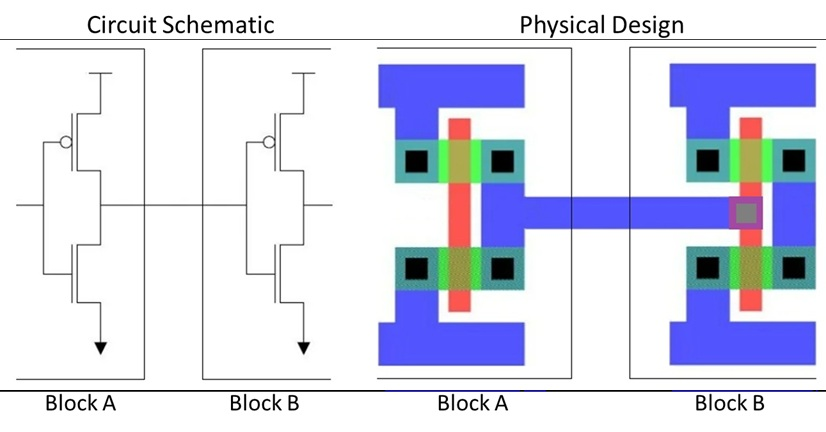
\includegraphics[width=0.9\linewidth]{figures/LayoutExample.jpg}
    \caption{Circuit Example}
    \label{fig:example}
\end{figure}

Typically, these metal wires are drawn to meet the minimum width requirements in the design rules for the manufacturing process.  However, if a design rule (DR) must be violated to avoid rework or save area, a waiver for the rule may be granted.  Design rules can be overkill for metal lines with little current flowing through them.  However, typical Reinforcement Learning-based place and route (P\&R) agents are constrained by the design rules.  Strategic design rule violations could potentially provide significant area savings without a significant impact on reliability. The key is to know which connection wires can violate the rules without sacrificing reliability.

\subsection{Strategic DR Violation}
\label{subsec:strategic_dr_violation}

The solution is to provide the Reinforcement Learning (RL) agent with the current flowing through each interconnection wire so that it can decide, based on current design calculations, which wires can be made narrower than the design rule.  Unfortunately, creating a simulation testbench for each circuit is expensive.  A solution to this expense is to use a Deep Learning model to estimate the current based on the design and process parameters, provide that information to the RL agent which then performs P\&R, then calculate the circuit reliability based on the routed layout.  This flowchart is shown in Figure \ref{fig:flowchart}.
  
\begin{figure}[H]
    \centering
    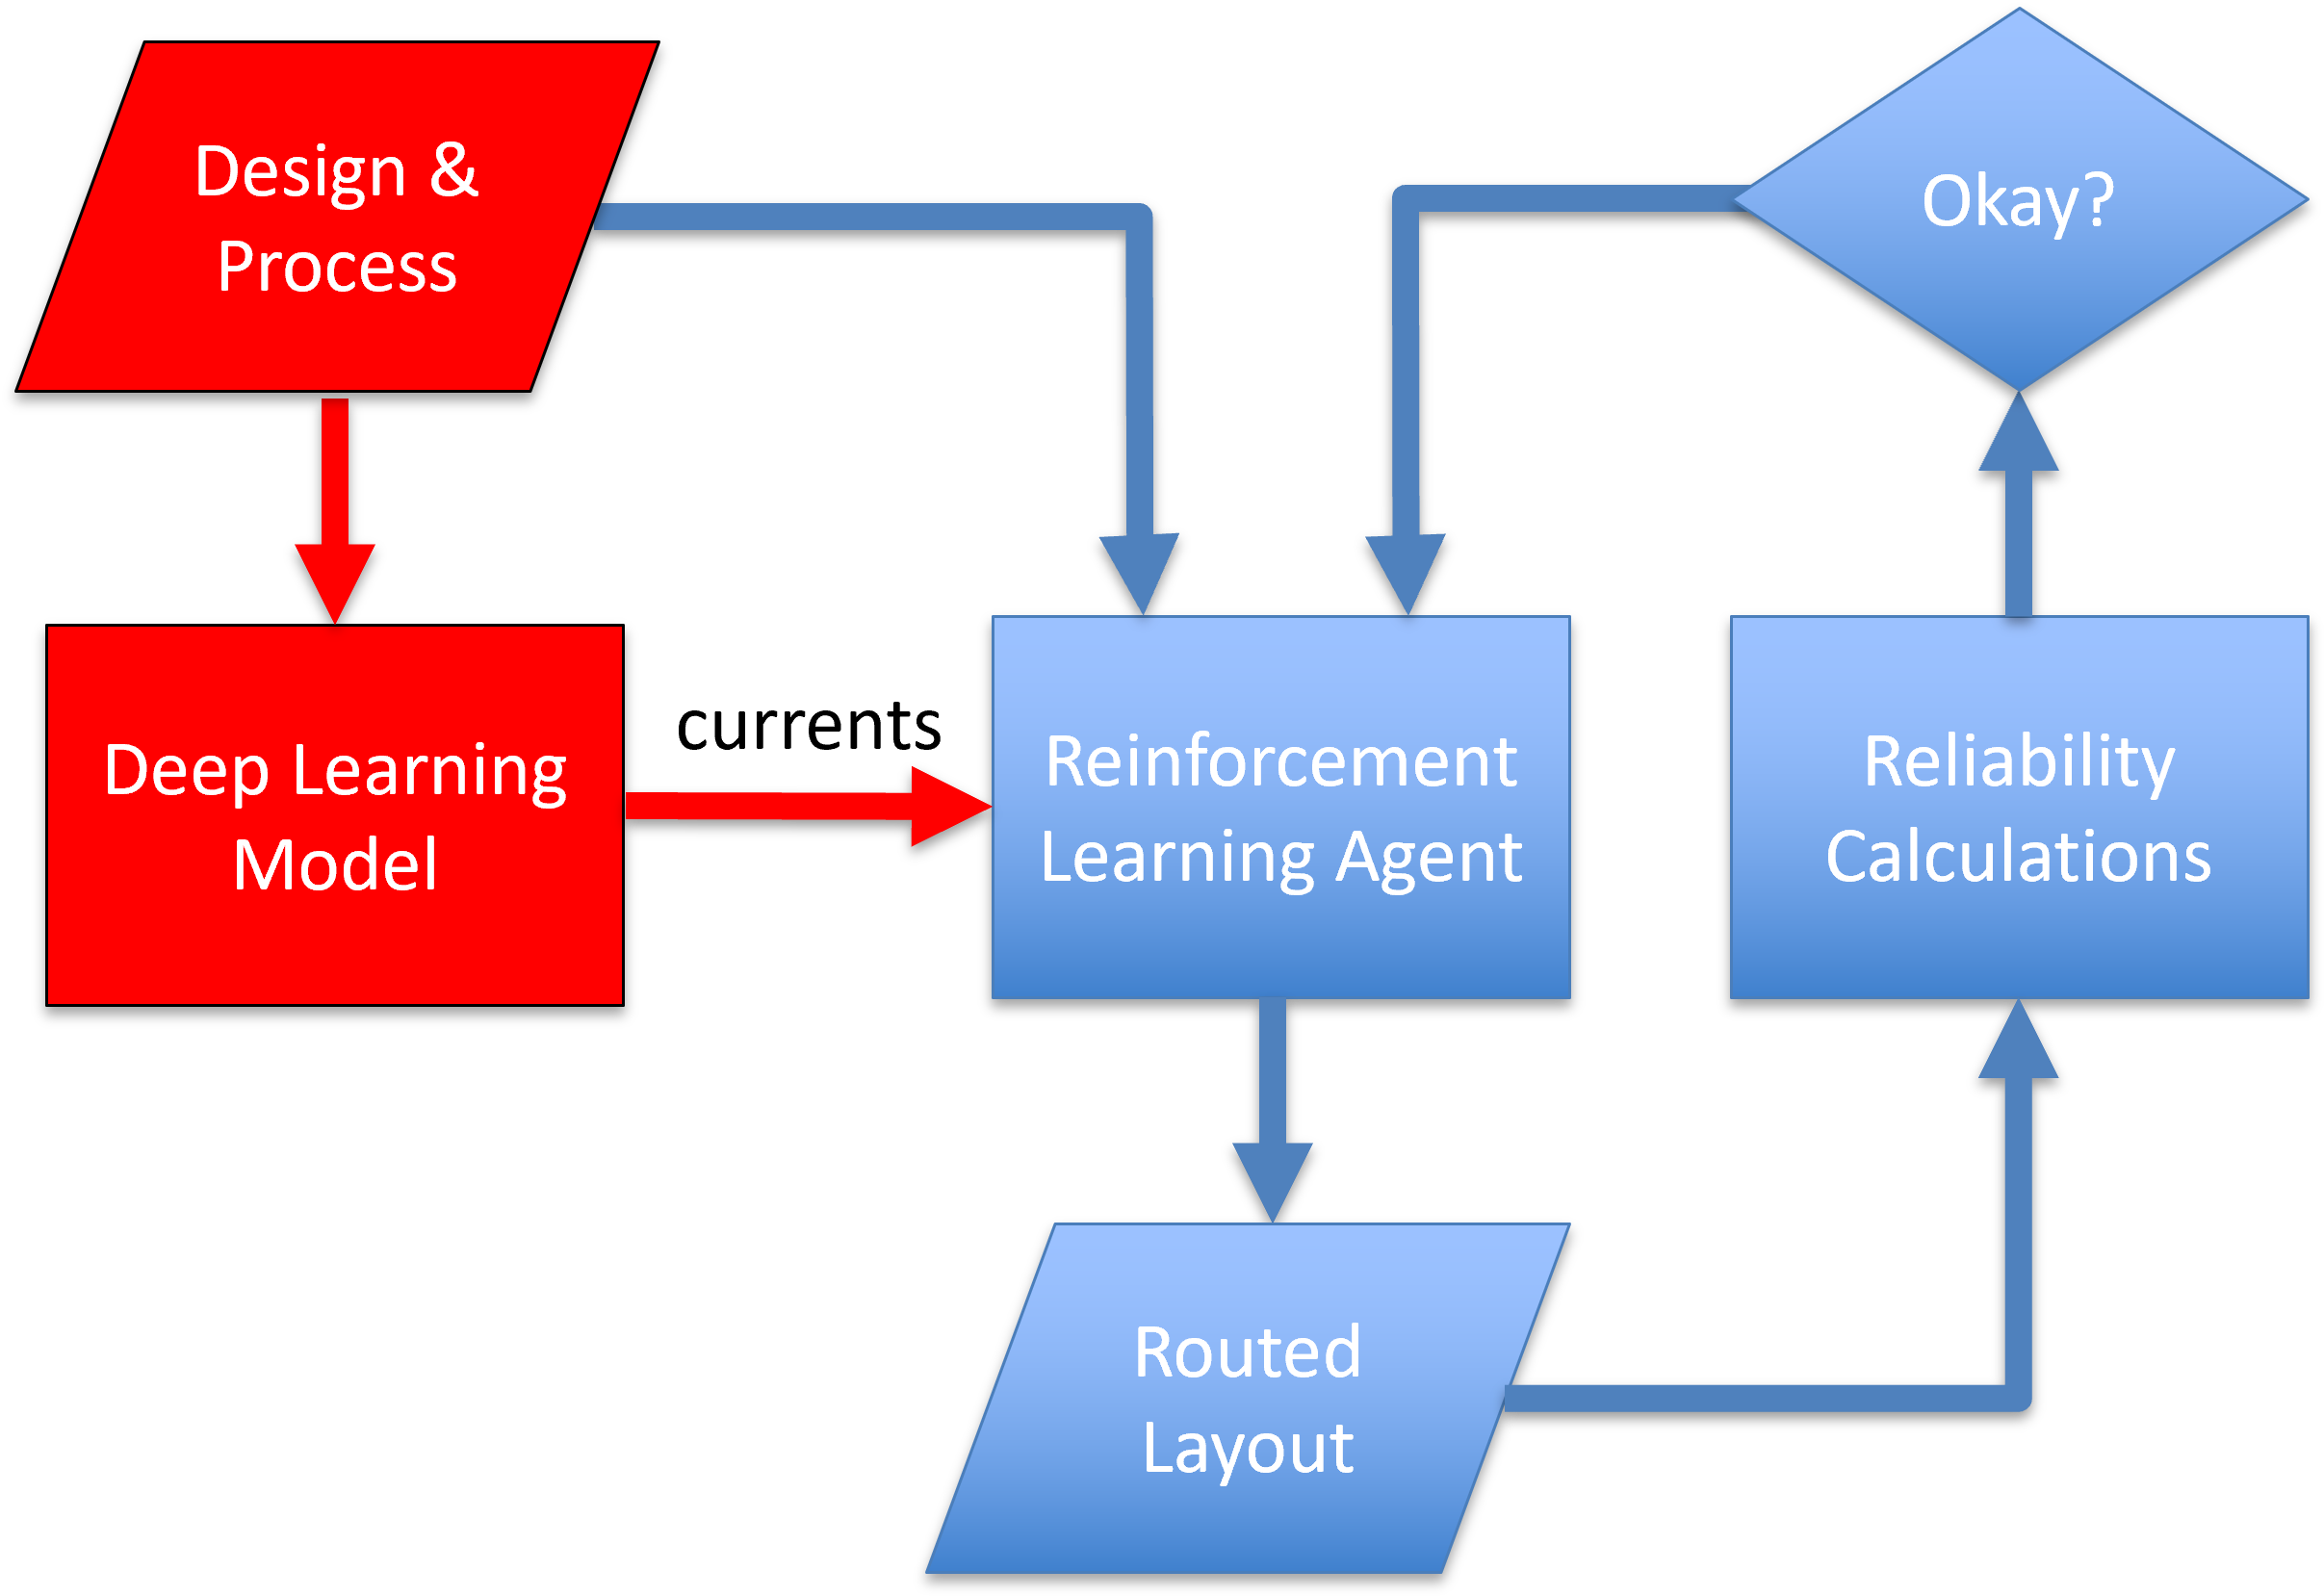
\includegraphics[width=0.8\linewidth]{figures/flowchart.png}
    \caption{System Flowchart}
    \label{fig:flowchart}
\end{figure}

The Deep Learning model needs to be trained on a dataset that contains simulation results representative of a circuit testbench. 

\subsection{Graph Neural Networks}
\label{subsec:gnn}

Graph neural networks are a type of neural network that uses a complete graph structure, rather than a single data sample, as one input. Mathematically, the graph is represented as a weighted adjacency matrix and a feature matrix whose rows are the feature vectors of each individual node in the graph. Learning can then be done to do classification or regression on node labels, edge weights, or an aggregate graph level \cite{DBLP:journals/corr/abs-1812-08434}.
GNNs can consist of many different types of layers, but the one that is most central to the concept is known generally as the message passing layer. This layer updates the features at each node, using information pulled from neighboring node features. For a general GNN this is not strictly defined, although the edges typically encode how the 'messages' are passed between nodes.

While there are many types of GNNs, Graph Attention Networks (GATs) extend the basic message-passing framework by learning a scalar attention weight for each directed edge, so the model can adaptively weight the influence of each neighbour rather than treating all connections equally \cite{velivckovic2018graph}. GATv2 \cite{brody2022how} corrects a rank-limitation in the original GAT by making the attention function strictly more expressive. In GATv2, the attention score for a given edge $(i, j)$ is computed as:
\begin{equation}
  e_{ij} = \mathbf{a}^{\top} \mathrm{LeakyReLU}\!\left(\mathbf{W}[\mathbf{h}_i \| \mathbf{h}_j]\right)
\end{equation}
where:\\

\begin{itemize}[nosep]
  \item $\mathbf{h}_i$ and $\mathbf{h}_j$ are the feature vectors of the source and target nodes, respectively
  \item $[\mathbf{h}_i \| \mathbf{h}_j]$ denotes concatenation of the two feature vectors
  \item $\mathbf{W}$ is a learnable weight matrix applied to the concatenated features
  \item $\mathrm{LeakyReLU}$ is a non-linear activation function
  \item $\mathbf{a}$ is a learnable vector that projects the result to a scalar attention score\\
\end{itemize}

This formulation allows the attention mechanism to depend jointly on both nodes, making it more expressive than the original GAT, which used separate projections and summed them before the nonlinearity. In a circuit graph, nodes represent transistors and interconnects whose relative contributions to downstream current vary depending on operating point; learned per-edge attention weights are therefore a natural fit compared to the uniform aggregation of a plain GCN \cite{DBLP:journals/corr/KipfW16}.

\subsection{Related Work}
\label{subsec:related_work}

There is already a large amount of existing literature on the topic of GNNs. For circuits specifically, El Sayed et al \cite{10.1145/3769081} conduct a survey on GNNs as tools in circuit design, although their scope is considerably broader than our own, discussing not just physical design but other applications such as logic design and synthesis. For direct application, Mirhoseini et al use edge-based GCNs to solve optimization problems in physical design \cite{Mirhoseini2021}. Their work once again differs from ours in the sense that the scope is much broader. Additionally, their approach differs in that they use deep reinforcement learning, while this is a simpler supervised learning approach.\\

The remainder of this report is organized as follows: Section~\ref{sec:datasets} describes dataset generation, including the circuit description, simulation methodology, and the datasets that were created; Section~\ref{sec:tech_approach} details the technical approach, including the Graph Neural Network and training procedure; Section~\ref{sec:experiment} presents the experimental design and results; and Section~\ref{sec:conclusion} provides the main conclusions and future work. The source code is in the Appendix.

\section{Datasets}
\label{sec:datasets}

The first step toward creating a dataset is to choose a test circuit.  For this project, the test circuit is a Cascaded CMOS Inverter Chain, as shown in Figure \ref{fig:2inv}.  The Spice netlist (\label{netlist:2inv}) is in the Appendix.  The target node, which represents the connection between two circuit blocks, is between them. Functionally, it is as simple as the circuit shown in Figure \ref{fig:example}, but requires additional elements related to the testbench in order to capture the simulation results necessary to generate the dataset.  The description of each element is below.

\begin{figure}[H]
    \centering
    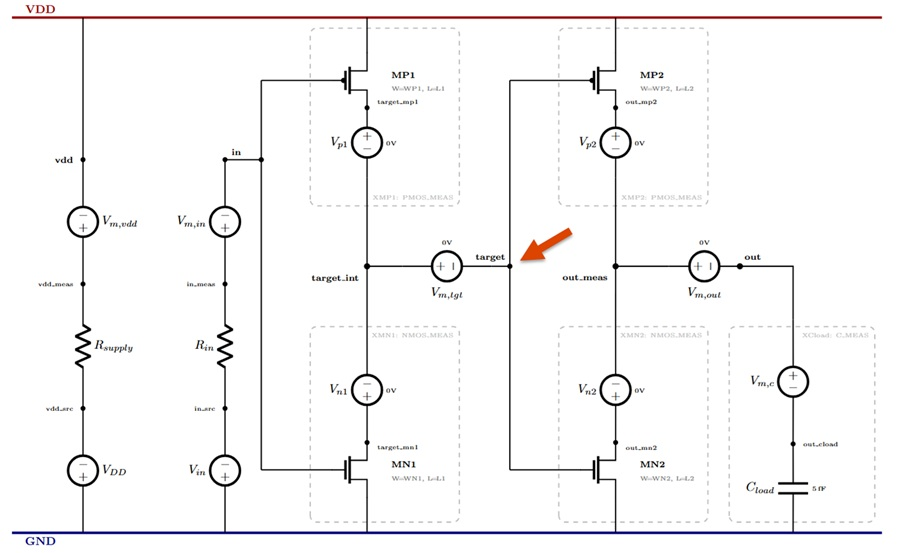
\includegraphics[width=1\linewidth]{figures/2inv_tb.jpg}
    \caption{Cascaded Inverter Testbench (2inv.sp)}
    \label{fig:2inv}
\end{figure}

\subsection{Circuit Description}
\label{subsec:circuit_description}

The testbench is comprised of transistors, subcircuits, measurement sources, and supply and input sources.  The transistors are what make up the inverters.  The rest of the elements are to facilitate measurement for data capture.  A description of each element is below.\\

\noindent \textbf{\normalsize Transistors}
\begin{itemize}[nosep]
  \item \textit{MP1} (PMOS, W=WP1, L=L1) is the pull-up transistor of the \emph{driver inverter} (INV1). When the input is low, MP1 charges the \texttt{target} node toward VDD. Its width WP1 and length L1 are swept across the design space.
  \item \textit{MN1} (NMOS, W=WN1, L=L1) is the pull-down transistor of the driver inverter. When the input is high, MN1 discharges \texttt{target} toward ground. Together with MP1, it sets the switching threshold and transition speed of INV1.
  \item \textit{MP2} (PMOS, W=WP2, L=L2) is the pull-up transistor of the \emph{load inverter} (INV2). Driven by the \texttt{target} node, it charges the \texttt{out} node. Its dimensions WP2 and L2 are independently swept.
  \item \textit{MN2} (NMOS, W=WN2, L=L2) is the pull-down transistor of the load inverter. Together with MP2, it presents a realistic capacitive and resistive load to the driver inverter, which directly affects the peak current drawn from VDD.\\
\end{itemize}

\noindent \textbf{\normalsize Subcircuits}
\begin{itemize}[nosep]
  \item \textit{XMP1: PMOS\_MEAS} (contains MP1 + $V_{p1}$) wraps the PMOS transistor with a 0\,V measurement voltage source ($V_{p1}$) in series with its drain. This allows SPICE to report the instantaneous drain current of MP1 as a branch current without disturbing the circuit.
  \item \textit{XMN1: NMOS\_MEAS} (contains MN1 + $V_{n1}$) uses the same technique for the NMOS transistor of INV1, enabling measurement of MN1's drain current via $V_{n1}$.
  \item \textit{XMP2: PMOS\_MEAS} (contains MP2 + $V_{p2}$) is the rain current measurement wrapper for MP2 in the load inverter.
  \item \textit{XMN2: NMOS\_MEAS} (contains MN2 + $V_{n2}$) is the rain current measurement wrapper for MN2 in the load inverter.
  \item \textit{XCload: C\_MEAS} (contains $C_{load}$ + $V_{m,c}$) wraps the 5\,fF load capacitor with a 0\,V measurement source. This captures the current flowing into the capacitive load, representing the dynamic charging/discharging current that a downstream stage would see.\\
\end{itemize}

\noindent \textbf{\normalsize Measurement Sources (0\,V)}
\begin{itemize}[nosep]
  \item \textit{$V_{m,vdd}$} (Vmeas\_vdd) measures the total current drawn from the VDD supply rail. Its peak value (\texttt{I\_vdd}) captures supply current behavior relevant to power integrity and IR-drop risk.
  \item \textit{$V_{m,in}$} (Vmeas\_in) measures the current delivered by the input source. Captures gate-tunneling and capacitive charging currents at the input node (\texttt{I\_in}).
  \item \textit{$V_{m,tgt}$} (Vmeas\_target) measures the current flowing from the driver inverter's output node (\texttt{target\_int}) to the load inverter's gate (\texttt{target}). Records \texttt{I\_target}, the primary prediction target for the DL model, reflecting the inter-stage drive current.
  \item \textit{$V_{m,out}$} (Vmeas\_out) measures the current at the output of the load inverter (\texttt{I\_out}), capturing the current flowing into the load capacitor path.
  \item \textit{$V_{p1}$, $V_{n1}$, $V_{p2}$, $V_{n2}$} is internal to PMOS\_MEAS / NMOS\_MEAS subcircuits. Each measures the drain current of its respective transistor, enabling per-device current attribution.
  \item \textit{$V_{m,c}$} is internal to C\_MEAS. Measures the capacitor charging current, distinguishing it from resistive leakage paths.\\
\end{itemize}

\noindent \textbf{\normalsize Supply and Input Sources}
\begin{itemize}[nosep]
  \item \textit{$V_{DD}$} is the DC voltage source providing the supply voltage. The value is swept across the design space to capture voltage-dependent behavior.
  \item \textit{$R_{supply}$} is a small series resistance (0.01\,$\Omega$) in the VDD path, modeling interconnect resistance and aiding convergence.
  \item \textit{$V_{in}$} is the pulsed voltage source (PULSE) generating the switching stimulus. Rise/fall times are 20\,ps; pulse width is 1\,ns with a 2\,ns period.
  \item \textit{$R_{in}$} is a small series resistance (0.01\,$\Omega$) in the input path, matching the VDD path topology.\\
\end{itemize}

The goal of the simulation is to measure the max voltage and peak current at each node in circuit, so it can be added to the dataset.  The nodes are described below.

\begin{itemize}[nosep]
  \item \textit{vdd} is a regulated supply rail, downstream of $V_{m,vdd}$. Voltage \texttt{V\_vdd} is recorded to verify supply integrity; current through $V_{m,vdd}$ gives the supply current target.
  \item \textit{in} is the gate input to INV1, downstream of $V_{m,in}$. Driven by a PULSE source ($V_{in}$) through $R_{in}$. Voltage \texttt{V\_in} and current \texttt{I\_in} are recorded.
  \item \textit{target\_int} is an internal output of INV1 (junction of MP1 and MN1 drain paths), before the measurement source $V_{m,tgt}$.
  \item \textit{target} is the gate input to INV2, downstream of $V_{m,tgt}$. Voltage \texttt{V\_target} and current \texttt{I\_target} are recorded. This is the inter-stage node whose transition drives the peak supply current.
  \item \textit{out\_meas} is an internal output of INV2 (junction of MP2 and MN2 drain paths), before $V_{m,out}$.
  \item \textit{out} is the final output node, downstream of $V_{m,out}$. Voltage \texttt{V\_out} and current \texttt{I\_out} are recorded.
  \item \textit{GND} (node 0) is the global ground reference. \texttt{I\_gnd} is derived by Kirchhoff's current law as the negative sum of all other node currents.\\
\end{itemize}

Table \ref{tab:columns} below shows the simulation results that will be captured as features in the dataset.

\begin{table*}
    \centering
    \scalebox{1}{
        \begin{tabular}{lll}
        \centering
        \textbf{Feature} & \textbf{Source} & \textbf{Description} \\
        \hline
        \texttt{V\_vdd}    & $V_{m,vdd}$, node vdd      & Peak voltage at VDD rail \\
        \texttt{V\_in}     & $V_{m,in}$, node in        & Peak voltage at input \\
        \texttt{V\_out}    & $V_{m,out}$, node out      & Peak voltage at output \\
        \texttt{V\_gnd}    & node 0                     & Ground reference (always 0) \\
        \texttt{V\_target} & $V_{m,tgt}$, node target   & Peak voltage at inter-stage node \\
        \texttt{I\_vdd}    & $V_{m,vdd}$ branch         & Peak supply current \\
        \texttt{I\_in}     & $V_{m,in}$ branch          & Peak input current \\
        \texttt{I\_out}    & $V_{m,out}$ branch         & Peak output current \\
        \texttt{I\_gnd}    & Kirchhoff (derived)        & Ground return current \\
        \texttt{I\_target} & $V_{m,tgt}$ branch         & \textbf{Peak inter-stage current (prediction target)} \\
        \hline
        \end{tabular}
    }
    \caption{Simulation Results as Dataset Features}
    \label{tab:columns}
\end{table*}

\subsection{Simulation Methodology}
\label{subsec:simulation_methodology}

The dataset was generated by simulating, using ngspice, the circuit testbench across different process models, process corners and skews, and transistor sizes. Each simulation represents a unique combination of process technology, operating conditions, device asymmetry, and circuit parameters.  These variations are described below.\\

\textbf{\normalsize Process Models (9 variations)} \cite{ptm_umn_models}. The simulation covers nine different semiconductor process technologies:

\begin{itemize}[nosep]
\item \textit{22nm HP:} Low threshold voltage, thin oxide for high performance 22nm node
\item \textit{22nm LP:} Higher threshold voltage for reduced leakage and low power 22nm node
\item \textit{32nm HP:} High performance 32nm node
\item \textit{32nm LP:} Low power 32nm node
\item \textit{45nm HP:} High performance 45nm node
\item \textit{45nm LP:} Low power 45nm node
\item \textit{65nm Bulk:} Traditional CMOS bulk process (neither HP nor LP)
\item \textit{90nm Bulk:} Mature bulk technology (neither HP nor LP)
\item \textit{130nm Bulk:} Legacy bulk process (neither HP nor LP)\\
\end{itemize}

\textbf{\normalsize PVT Corners (5 variations)}. Process, Voltage, Temperature combinations for comprehensive operating conditions:

\begin{itemize}[nosep]
\item \textit{Typical:} Nominal operating conditions
\item \textit{Slow:} Conservative: Low voltage, high temperature
\item \textit{Fast:} Aggressive: High voltage, low temperature
\item \textit{Hot:} High temperature stress testing
\item \textit{Cold:} Low temperature operation\\
\end{itemize}

\textbf{\normalsize Process Skew Corners (5 variations)}. Device asymmetry variations capturing realistic NMOS/PMOS device mismatches:

\begin{itemize}[nosep]
\item \textit{TT:} Balanced device performance
\item \textit{FF:} Both devices fast (high performance)
\item \textit{SS:} Both devices slow (low leakage)
\item \textit{FS:} Asymmetric: affects rise vs fall times
\item \textit{SF:} Asymmetric: affects fall vs rise times\\
\end{itemize}

\textbf{\normalsize Monte Carlo Device Parameters}. For each combination above, the following parameters are randomly sampled:

\begin{itemize}[nosep]
\item \textit{WN1, WN2:} NMOS transistor widths (process-specific ranges)
\item \textit{WP1, WP2:} PMOS transistor widths (process-specific ranges)
\item \textit{L1, L2:} Channel lengths, 20nm-600nm (node dependent)
\item \textit{VDD:} Supply voltage, 0.7V-2.0V (node dependent)
\item \textit{TEMP:} Operating temperature, -20°C to 125°C
\item \textit{Example 22nm ranges:} W: 0.2$\mu$m - 8$\mu$m, L: 20nm - 200nm\\
\end{itemize}

\subsection{Dataset 1}
\label{subsec:dataset1}

Dataset 1 was generated using only a single process model, 22nm\_HP.pm.  This was to determine whether the model could be accurate on a smaller feature size.  This means that for every combination of device parameters, 25 (5 corners x 5 skews) simulations were run.  Figure \ref{fig:ds1} shows a single instance of Dataset 1.  The dataset contains 100,000 instances.

ID is the instance number.  Design is the circuit.  Even though it’s the same for every instance, it makes sense to include this in the dataset because of future work will include multiple designs.  Size and Option are the process.  22 is the minimum feature size in nanometers and HP means it’s the High Performance version of the model.  This is as opposed to LP, which stands for Low Power.  PVT and Skew are simulation corners.  PVT is Process, Voltage, and Temperature.  The voltage is the supply voltage.  Skew is how the transistors perform.  SS means both N-type and P-type are slow.  Skew can also be fast/fast, fast/slow, slow/fast, and typical/typical.  The Ws and Ls are transistor sizes.  For example, WN1 is the gate width of the N-type transistor in the first stage.  Similarly for the others.  It’s typical for the N-type and P-type transistors to have the same gate length, so there are only two lengths.  VDD is the supply voltage and Temp is the temperature.  The rest are the voltages and current for the nodes, the last being the target current the model is going to predict.

\begin{figure}[H]
    \centering
    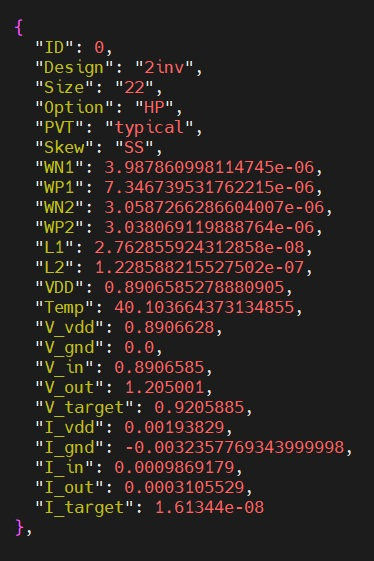
\includegraphics[width=0.6\linewidth]{figures/dataset.json.jpg}
    \\[2ex]
    \caption{Dataset 1 in JSON Format}
    \label{fig:ds1}
\end{figure}

\subsection{Dataset 2}
\label{subsec:dataset2}

Dataset 2 was generated using all 12 process models.  This was to determine whether the model could be generalized to a larger feature size.  This means that for every combination of device parameters, 25 (5 corners x 5 skews) simulations were run.  Figure \ref{fig:ds2} shows a single instance of dataset 2.  The dataset contains 112,500 instances.

\begin{figure}[H]
    \centering
    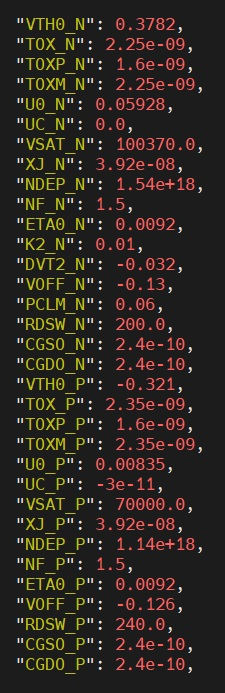
\includegraphics[width=0.4\linewidth]{figures/dataset2.json.jpg}
    \\[2ex]
    \caption{Part of Dataset 2}
    \label{fig:ds2}
\end{figure}

The second dataset has all of the same features as the first dataset, plus some more.  The additional features are parameters that change between process models.  The parser automatically removes any parameter that doesn’t change at all.  Some parameters don’t change much, so they may need to be pruned.  Also, because some of the numbers are huge and time are minuscule, they may need to be normalized. The new features in Dataset 2 are below.  Note that they have \_N and \_P versions.  This is because the parameters differ for N-type and P-type transistors.

\textbf{VTH0:} Zero-bias threshold voltage (``on'' voltage).
\textbf{VOFF:} Adjusts the subthreshold current curve so simulation matches measured data.
\textbf{TOX / TOXP / TOXM:} Gate dielectric thickness, which determines gate capacitance.
\textbf{U0:} Controls carrier mobility, which determines current drive.
\textbf{UC:} Mobility degradation coefficient.
\textbf{VSAT:} Carrier velocity saturation limit.
\textbf{XJ:} Junction depth of source/drain diffusion.
\textbf{NDEP:} Channel doping concentration.
\textbf{DVT2:} Second-order short-channel threshold roll-off parameter.
\textbf{ETA0:} Controls how drain voltage lowers the threshold voltage.
\textbf{K2:} Second-order body effect coefficient.
\textbf{PCLM:} Controls channel length modulation.
\textbf{RDSW:} Source/drain sheet resistance per width.
\textbf{CGSO / CGDO:} Gate-to-source overlap capacitance.
\textbf{NF:} Number of gate fingers.

\section{Technical Approach}
\label{sec:tech_approach}

The technical approach was to implement a Graph Attention Network (GAT) for regression on circuit edge weights, where the circuit is represented as a graph with nodes corresponding to circuit components (such as transistors and interconnects) and edges representing electrical connections. Each node is assigned a feature vector encoding its physical and electrical properties. The GAT learns to incorporate information from neighboring nodes using attention mechanisms, allowing it to adaptively weight the influence of each neighbor based on both the source and target node features. The model is trained to predict the peak current for the relevant edge (I\_target), enabling accurate current estimation without requiring full SPICE simulations.

\subsection{Implementation}
\label{subsec:implementation}

Our training algorithm was implemented in Python using PyTorch and the PyG library \cite{PyG_Documentation} for GATv2Conv layers. Experiment tracking is performed with Weights \& Biases. The main training and experiment orchestration code is in \texttt{python/sweep.py}, with supporting data and model code in \texttt{python/dataset.py}, \texttt{python/gan.py}, and \texttt{python/graph.py} (see Appendix). The code repository can be found here: \url{https://github.com/YosemiteSamurai/CurrentPrediction}.

\subsection{Model Architecture}
\label{subsec:model_architecture}

To predict current values, regression on the graph's edge weights with a GATv2 network \cite{brody2022how} are used. For this problem, the graphs have been designed such that our training is entirely supervised. The model consists of three stages of \texttt{GATv2Conv} layers \cite{PyG_Documentation}:\\

\begin{enumerate}[nosep]
  \item An input layer mapping node features to a 64-dimensional hidden space, using 4 attention heads whose outputs are averaged.
  \item Three hidden layers of the same width and head configuration, each followed by an ELU activation.
  \item An output layer with 4 heads whose outputs are \emph{concatenated}, producing a 64-dimensional node embedding (16 dimensions per head).\\
\end{enumerate}

These three stages work together as follows:

\subsubsection{Input Layer}
\label{subsubsec:input_layer}

The input layer takes the raw node features, which may vary in dimension depending on the dataset, and projects them into a fixed 64-dimensional hidden space. This is accomplished using a GATv2Conv layer with 4 attention heads. The choice of 4 attention heads is a balance between model expressiveness and computational efficiency. Using multiple heads allows the model to attend to different aspects of the neighborhood structure simultaneously, capturing diverse patterns in the data. Empirically, 4 heads provided sufficient capacity for the circuit prediction task without incurring excessive computational cost or overfitting. Fewer heads (e.g., 3) may limit the model's ability to capture complex relationships, while more heads (e.g., 5 or more) increase memory and computation without a clear gain in performance for this dataset.

Each head computes its own attention-weighted aggregation of neighboring node features, and the outputs of the 4 heads are averaged. In the GATv2Conv implementation, each attention head produces an output vector of size 64. When using 4 heads with averaging, the outputs from all heads are summed and divided by 4, resulting in a single 64-dimensional vector per node. This is in contrast to concatenation, which would produce a 256-dimensional output (4 heads $\times$ 64 dimensions each). Averaging preserves the original hidden size, ensuring the output remains 64-dimensional, providing a consistent embedding size for all nodes regardless of the original feature dimension.

The hidden size of 64 is a common choice in graph neural networks, providing enough capacity to encode rich node representations while keeping the model tractable for large graphs. It is large enough to capture the relevant features and interactions in the circuit graphs, but not so large as to risk overfitting or slow down training significantly. This value was selected based on standard practice and preliminary experiments.

Consistent embedding size is crucial because subsequent layers in the network expect a fixed-size input for every node, regardless of the original feature vector's dimension. This uniformity allows the model to process graphs with nodes of varying feature sets (e.g., different circuit components) and ensures compatibility with batch processing and downstream layers. By projecting all node features into the same 64-dimensional space, the model can generalize across different node types and datasets, facilitating transfer learning and robust performance.

\subsubsection{Hidden Layers}
\label{subsubsec:hidden_layers}

The next three layers are also GATv2Conv layers, each with 4 attention heads and a hidden size of 64. The choice of three hidden layers is a balance between model depth and the risk of overfitting or vanishing gradients. With each additional layer, the model can aggregate information from nodes that are further away in the graph, enabling it to capture more complex dependencies.  The rationale having 4 attention heads is similar to the input layer: multiple heads allow the model to capture diverse patterns and relationships in the graph. Four heads provide a good trade-off between expressiveness and computational cost, as validated by experiments. Using the same number of heads across layers also simplifies the architecture and ensures consistent dimensionality.

After each layer, an Exponential Linear Unit (ELU) activation is applied to introduce nonlinearity. Nonlinearity is essential in neural networks to allow the model to learn complex, non-linear relationships in the data. Without nonlinear activations, the network would be limited to learning only linear transformations, regardless of its depth. The Exponential Linear Unit (ELU) is chosen because it helps mitigate the vanishing gradient problem, speeds up learning, and can produce negative outputs, which may be beneficial for representing certain circuit features. ELUs often lead to faster convergence and better generalization compared to ReLU or other activations in some graph neural network applications.

The hidden layers allow the model to iteratively refine node representations by aggregating information from increasingly distant neighbors in the graph. The attention mechanism enables the model to focus on the most relevant nodes for each prediction, which is especially important in circuit graphs where certain nodes (such as supply rails or transistors) play more critical roles than others.

While graph size can influence architectural choices, the decisions here are primarily based on standard practice in graph neural networks. The circuit graphs in this work are of moderate size, so three layers are sufficient to capture relevant dependencies without excessive depth. The number of attention heads and the use of ELU are chosen for their general effectiveness rather than being tightly coupled to graph size. For much larger or more complex graphs, deeper networks or different configurations might be explored.

\subsubsection{Output Layer}
\label{subsubsec:output_layer}

The final GATv2Conv layer also uses 4 attention heads, but instead of averaging their outputs, it concatenates them. The rationale for using 4 attention heads in the output layer is consistent with the earlier layers: multiple heads allow the model to capture different aspects of the node's neighborhood and learn a more nuanced representation. Four heads provide a good balance between model expressiveness and computational efficiency, as established in the input and hidden layers.

In the output layer, concatenation is used instead of averaging to preserve the unique information captured by each attention head. While averaging blends the outputs into a single vector (as in the input and hidden layers), concatenation retains the distinct features learned by each head, resulting in a richer and more expressive final embedding. This is particularly valuable for the final prediction, as it allows the decoder to leverage a broader set of features when estimating the target current. Concatenation increases the dimensionality (4 heads $\times$ 16 dimensions = 64), but this is intentional to maximize the information available for the final regression task.

This results in a 64-dimensional node embedding, with each head contributing 16 dimensions. The concatenated output provides a richer and more expressive representation, which is then used by the decoder to predict the target edge current. This design allows the model to capture a diverse set of features from different attention heads, improving its ability to generalize across different circuit configurations.\\

\subsection{Graphical Circuit Models}
\label{subsec:graphical_models}

Creating a graphical model of a circuit can be approached in several different ways.
In physics problems, a circuit is typically translated to graph form by treating partitions of wire with equal potential as the nodes.
For this case, however, it is preferable to encode circuit components as nodes to limit feature data to nodes and label data to edges, respectively. This allows the model to learn the relationship between component features and current flow, rather than relying on the model to infer the presence of components from patterns in the adjacency matrix. It also allows for more flexible modeling of complex circuit topologies, where multiple components may be connected in parallel or series, without needing to explicitly encode these configurations in the graph structure.

\subsection{Feature Engineering and Loss Function}
\label{subsec:feature_engineering}

Feature engineering encompasses all transformations applied to both input features and target labels to make the data suitable for model training (see Appendix, \texttt{python/dataset.py}). For the input features, two main strategies are used: (1) Convert descriptive parameters to numerical encodings, using their implied ordinality. For example, Skew is converted to a two-dimensional parameter describing the corner placement, and Option is converted to a one-dimensional parameter encoding low, medium, or high power. The PVT parameters are dropped due to redundancy with other numerical parameters. (2) To address imbalance in feature scale, features are standardized across the entire dataset to a mean of zero and variance of one. This prevents cases of exploding gradient during training.

For the target labels (currents), label normalization is performed as a specialized form of feature engineering. The five branch currents in the dataset span approximately six orders of magnitude (8\,pA to 46\,$\mu$A). Training directly on raw current values with MAPE or MAE loss produced unstable gradients and poor convergence on small-magnitude currents. To address this, all current labels are normalized using a two-step process:

\begin{equation}
  \hat{y} = \frac{\log_{10}(|I|) - \mu}{\sigma}
\end{equation}

where $\mu$ and $\sigma$ are computed from the flattened log-magnitudes of all current values across the full training set. This compresses the six-order dynamic range to a near-unit-scale output target. At evaluation time the prediction is inverse-transformed as $I = 10^{\hat{y}\,\sigma + \mu}$.  With log-normalized labels, standard L1 loss (mean absolute error) becomes equivalent to a log-space relative error:

\begin{equation}
  \mathcal{L} = \frac{1}{N}\sum_{i=1}^{N} \left| \hat{y}_i - y_i \right|
\end{equation}

Critically, the loss is computed \textit{only on I\_target edges}. At inference time the model receives only transistor dimensions and process/PVT parameters — no other branch currents are available. Masking the loss to I\_target ensures the gradient signal reflects the actual prediction objective and avoids dilution from the five other edge types (I\_vdd, I\_gnd, I\_in, I\_out, and their junction duplicates).

\subsection{Batching}
\label{subsec:batching}

In standard machine learning, all data samples (e.g., images) have the same shape.  However, in graph learning, each graph can have a different number of nodes and edges, so their feature and adjacency matrices have different sizes. Because of this inconsistency, it's not possible to use standard batching techniques. The solution is to merge all of the graphs in a batch into a single, larger ``super-graph'' by concatenating all of the node feature matrices vertically, then placing each graph's adjacency matrix along the diagonal of a large, block-diagonal matrix (with zeroes elsewhere). This way, the batch is represented as one large graph, and the GAN can process all graphs in the batch together efficiently. \cite{PyG_Documentation} (Batching implementation: see Appendix, \texttt{sweep.py} and \texttt{graph.py})
At low batch sizes typical problems with stability were observed and large batch sizes led to a notable increase in measured error, so a batch size of 32 was chosen as a balance between stability and training speed.

\subsection{Decoder}
\label{subsec:decoder}

After the GATv2 encoder processes the graph, each node is represented by a 64-dimensional embedding vector $\mathbf{z}_i$ that encodes its physical, electrical, and topological context. The decoder's job is to predict the current for each edge $(u, v)$ using these node embeddings.  To do this, the decoder constructs a feature vector for each edge by combining information from both endpoint nodes in several ways:

\begin{itemize}
  \item $\mathbf{z}_u$: Embedding of the source node (e.g., a transistor or interconnect)
  \item $\mathbf{z}_v$: Embedding of the target node
  \item $\mathbf{z}_u - \mathbf{z}_v$: Element-wise difference, capturing the relative relationship between the nodes
  \item $\mathbf{z}_u \odot \mathbf{z}_v$: Element-wise (Hadamard) product, capturing interactions between corresponding features
\end{itemize}

These four 64-dimensional vectors are concatenated to form a single 256-dimensional input vector for each edge:

\begin{equation}
  [\mathbf{z}_u \,\|\, \mathbf{z}_v \,\|\, \mathbf{z}_u - \mathbf{z}_v \,\|\, \mathbf{z}_u \odot \mathbf{z}_v] \in \mathbb{R}^{256}
\end{equation}

This design allows the decoder to leverage both the individual properties of each node and their pairwise relationships, which is important for accurately modeling current flow that depends on both local and contextual circuit features. The 256-dimensional edge feature vector is then passed through a two-layer multilayer perceptron (MLP):

\begin{itemize}
  \item \textbf{First layer:} Fully connected, 256 $\rightarrow$ 64, followed by a ReLU activation. This layer learns nonlinear combinations of the edge features.
  \item \textbf{Second layer:} Fully connected, 64 $\rightarrow$ 1, producing a single scalar output $\hat{y}_{uv}$, which is the predicted log-normalized current for that edge.
\end{itemize}

Mathematically, the decoder can be written as:
\begin{equation}
  \hat{y}_{uv} = \mathrm{MLP}\!\left([\mathbf{z}_u \,\|\, \mathbf{z}_v \,\|\, \mathbf{z}_u - \mathbf{z}_v \,\|\, \mathbf{z}_u \odot \mathbf{z}_v]\right)
\end{equation}

This approach is well-suited for edge regression tasks in graph neural networks, as it allows the model to flexibly capture both additive and multiplicative interactions between node features, as well as their differences, which can be critical for predicting physical quantities like current that depend on the relationship between two circuit elements. The use of a two-layer MLP provides sufficient capacity to model complex nonlinear dependencies while remaining computationally efficient.

\subsection{Optimization}
\label{subsec:optimization}

The model is trained with the Adam optimizer at an initial learning rate of $1 \times 10^{-4}$. A \texttt{ReduceLROnPlateau} scheduler halves the learning rate after 8 consecutive epochs without improvement in test loss, with a minimum learning rate of $1 \times 10^{-6}$. Training runs for 100 epochs with a batch size of 32 graphs, on a 70/30 train/test split of Dataset~1 (70,000 training, 30,000 test samples). Training is performed on an NVIDIA RTX~8000 GPU via the OSU College of Engineering HPC cluster.

\section{Experiment}
\label{sec:experiment}

The goal of our experiment is to directly compare two training regimes: one where the model is trained on Dataset~2 (multi-process, spanning nine manufacturing process technologies), and one where the model is trained on Dataset~1 (single process, 22\,nm HP only). This comparison is designed to answer two key questions:

\begin{enumerate}
    \item Can a GAN predict the current accurately enough to effectively replace a SPICE simulation, as shown in Figure \ref{fig:flowchart}?
    \item If so, can a single model generalize across all processes without sacrificing accuracy, or does there need to be a model per process?
\end{enumerate}

All experiments were tracked and visualized using Weights \& Biases (wandb): \url{https://wandb.ai/yosemitesamurai/CurrentPrediction}.

\subsection{Design}
\label{subsec:design}

All experiments use the block-inverter graph model (\texttt{block\_2inv}), 3 hidden GATv2 layers, hidden dimension 64, 4 attention heads, batch size 32, and initial learning rate $1\times10^{-4}$.

\subsection{Evaluation}
\label{subsec:evaluation}

The primary evaluation metric is Mean Relative Error (MRE) on I\_target in physical units (Amperes), computed on the held-out test set:
\begin{equation}
  \mathrm{MRE} = \frac{1}{N} \sum_{i=1}^{N} \left| \frac{I_{\mathrm{pred},i} - I_{\mathrm{true},i}}{I_{\mathrm{true},i}} \right|
\end{equation}
Predictions are inverse-transformed from log-normalized space before this calculation. MRE is evaluated \textbf{only on I\_target edges} — the only current available at inference time and the quantity of engineering interest. We also report test L1 loss in log-normalized space as a stable training diagnostic.

\subsection{Results}
\label{subsec:results}

We compare the performance of the model when trained on Dataset~2 (multi-process) versus Dataset~1 (single process). The central question is whether a single model can generalize across all process technologies, or if accuracy is fundamentally limited by the need to distinguish between process clusters. The following results and figures summarize the training dynamics, error metrics, and learning rate schedules for both datasets side by side.

Figure \label{fig:trainloss_compare} is the training loss (L1) over epochs for both Dataset~1 (single process) and Dataset~2 (multi-process). Figure \label{fig:mre_compare} is the mean relative error (MRE) on I\_target during training for both datasets. Figure \label{fig:lr_compare} is the learning rate schedule during training for both datasets.  All three figures were tracked and visualized with wandb.

\begin{figure}[H]
  \centering
  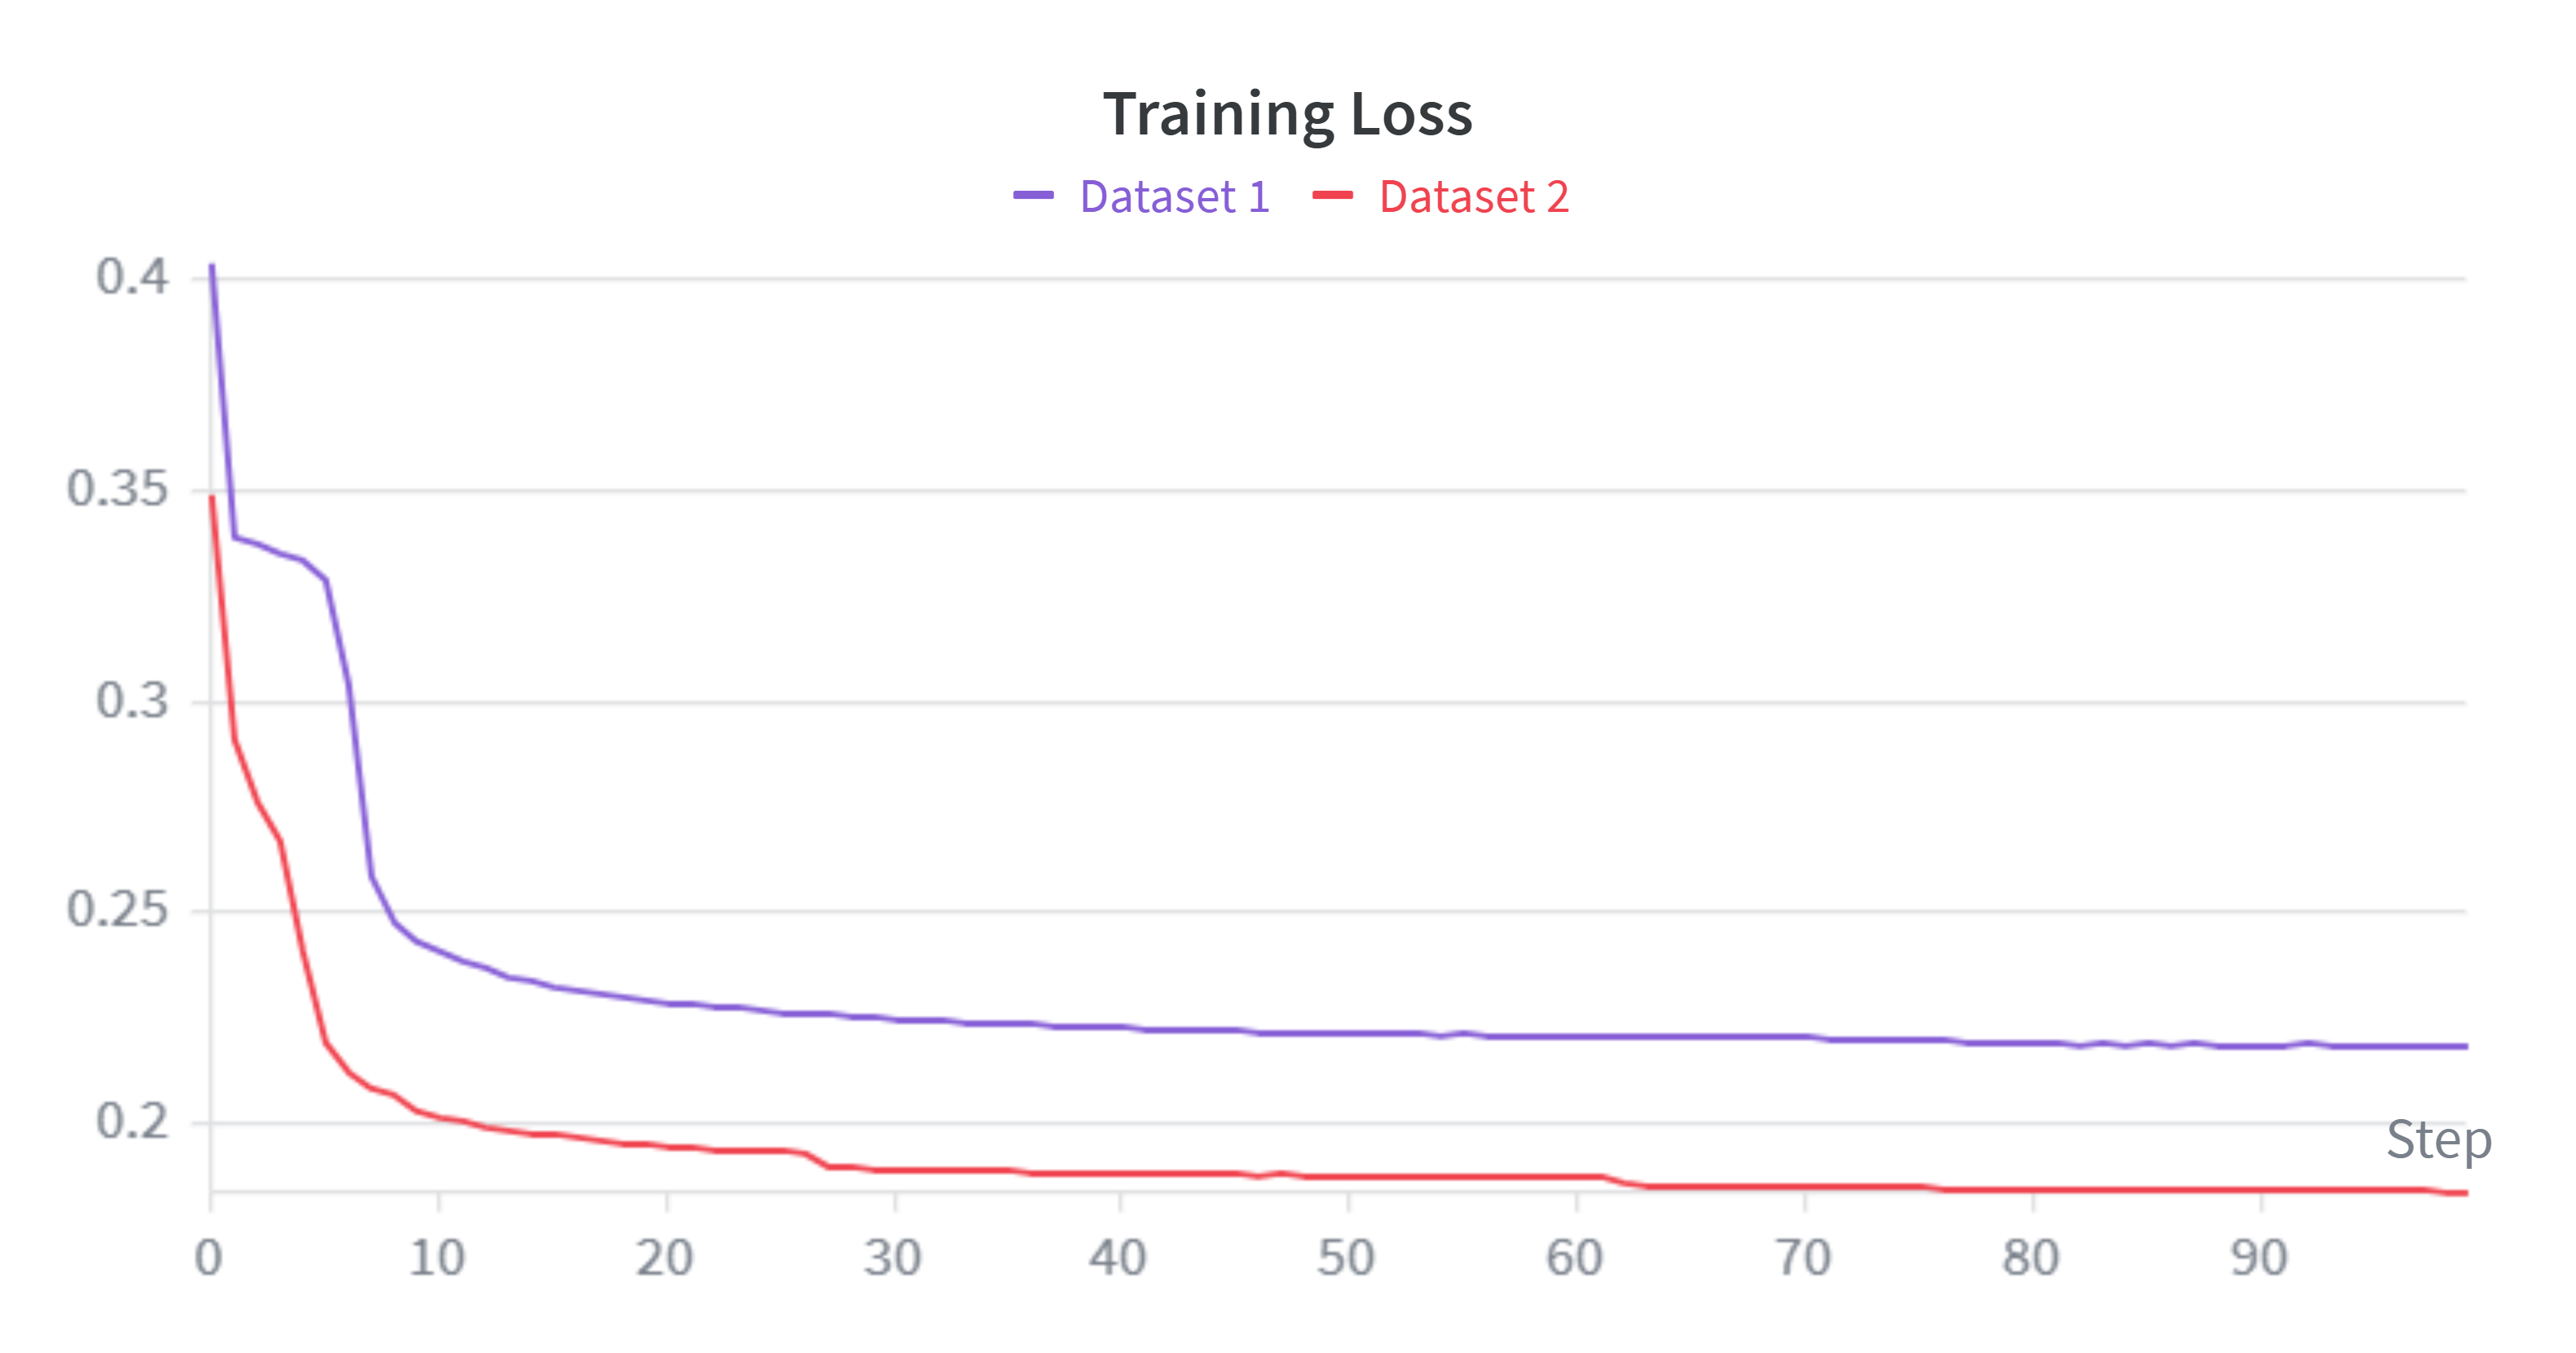
\includegraphics[width=0.95\linewidth]{figures/TrainingLoss.png}
  \caption{Training loss (L1) over epochs}
  \label{fig:trainloss_compare}
\end{figure}

\begin{figure}[H]
  \centering
  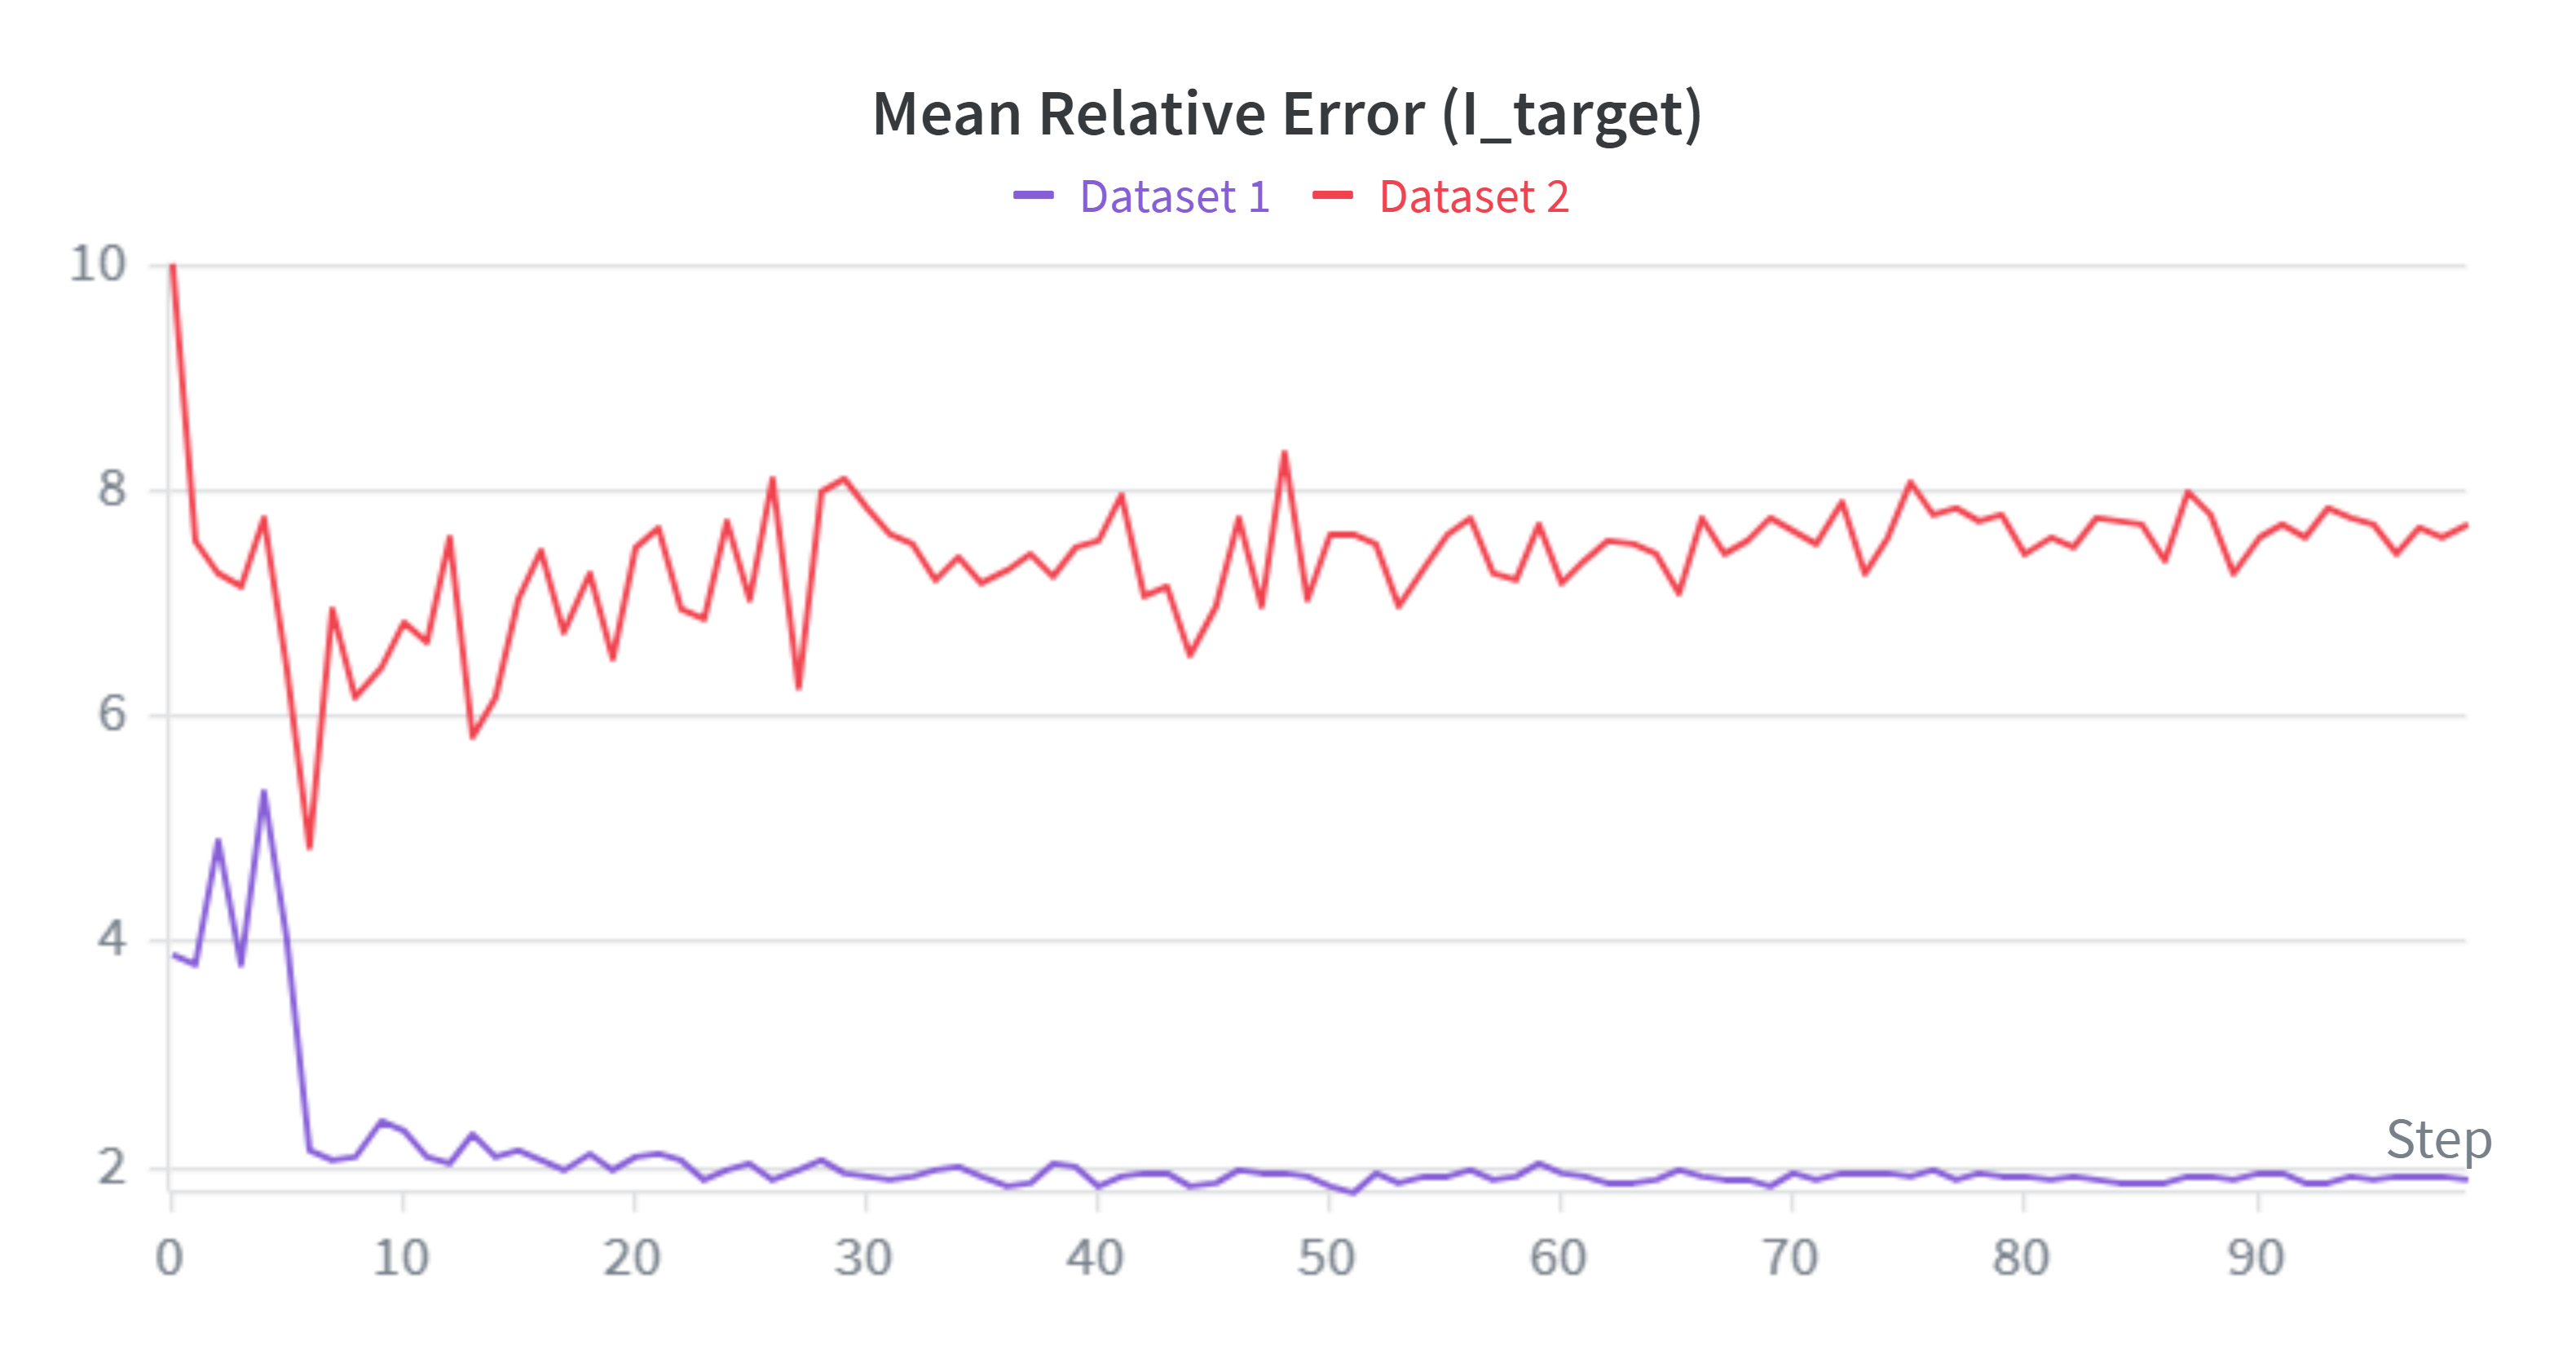
\includegraphics[width=0.95\linewidth]{figures/MeanRelativeError.png}
  \caption{Mean relative error (MRE) on I\_target}
  \label{fig:mre_compare}
\end{figure}

\begin{figure}[H]
  \centering
  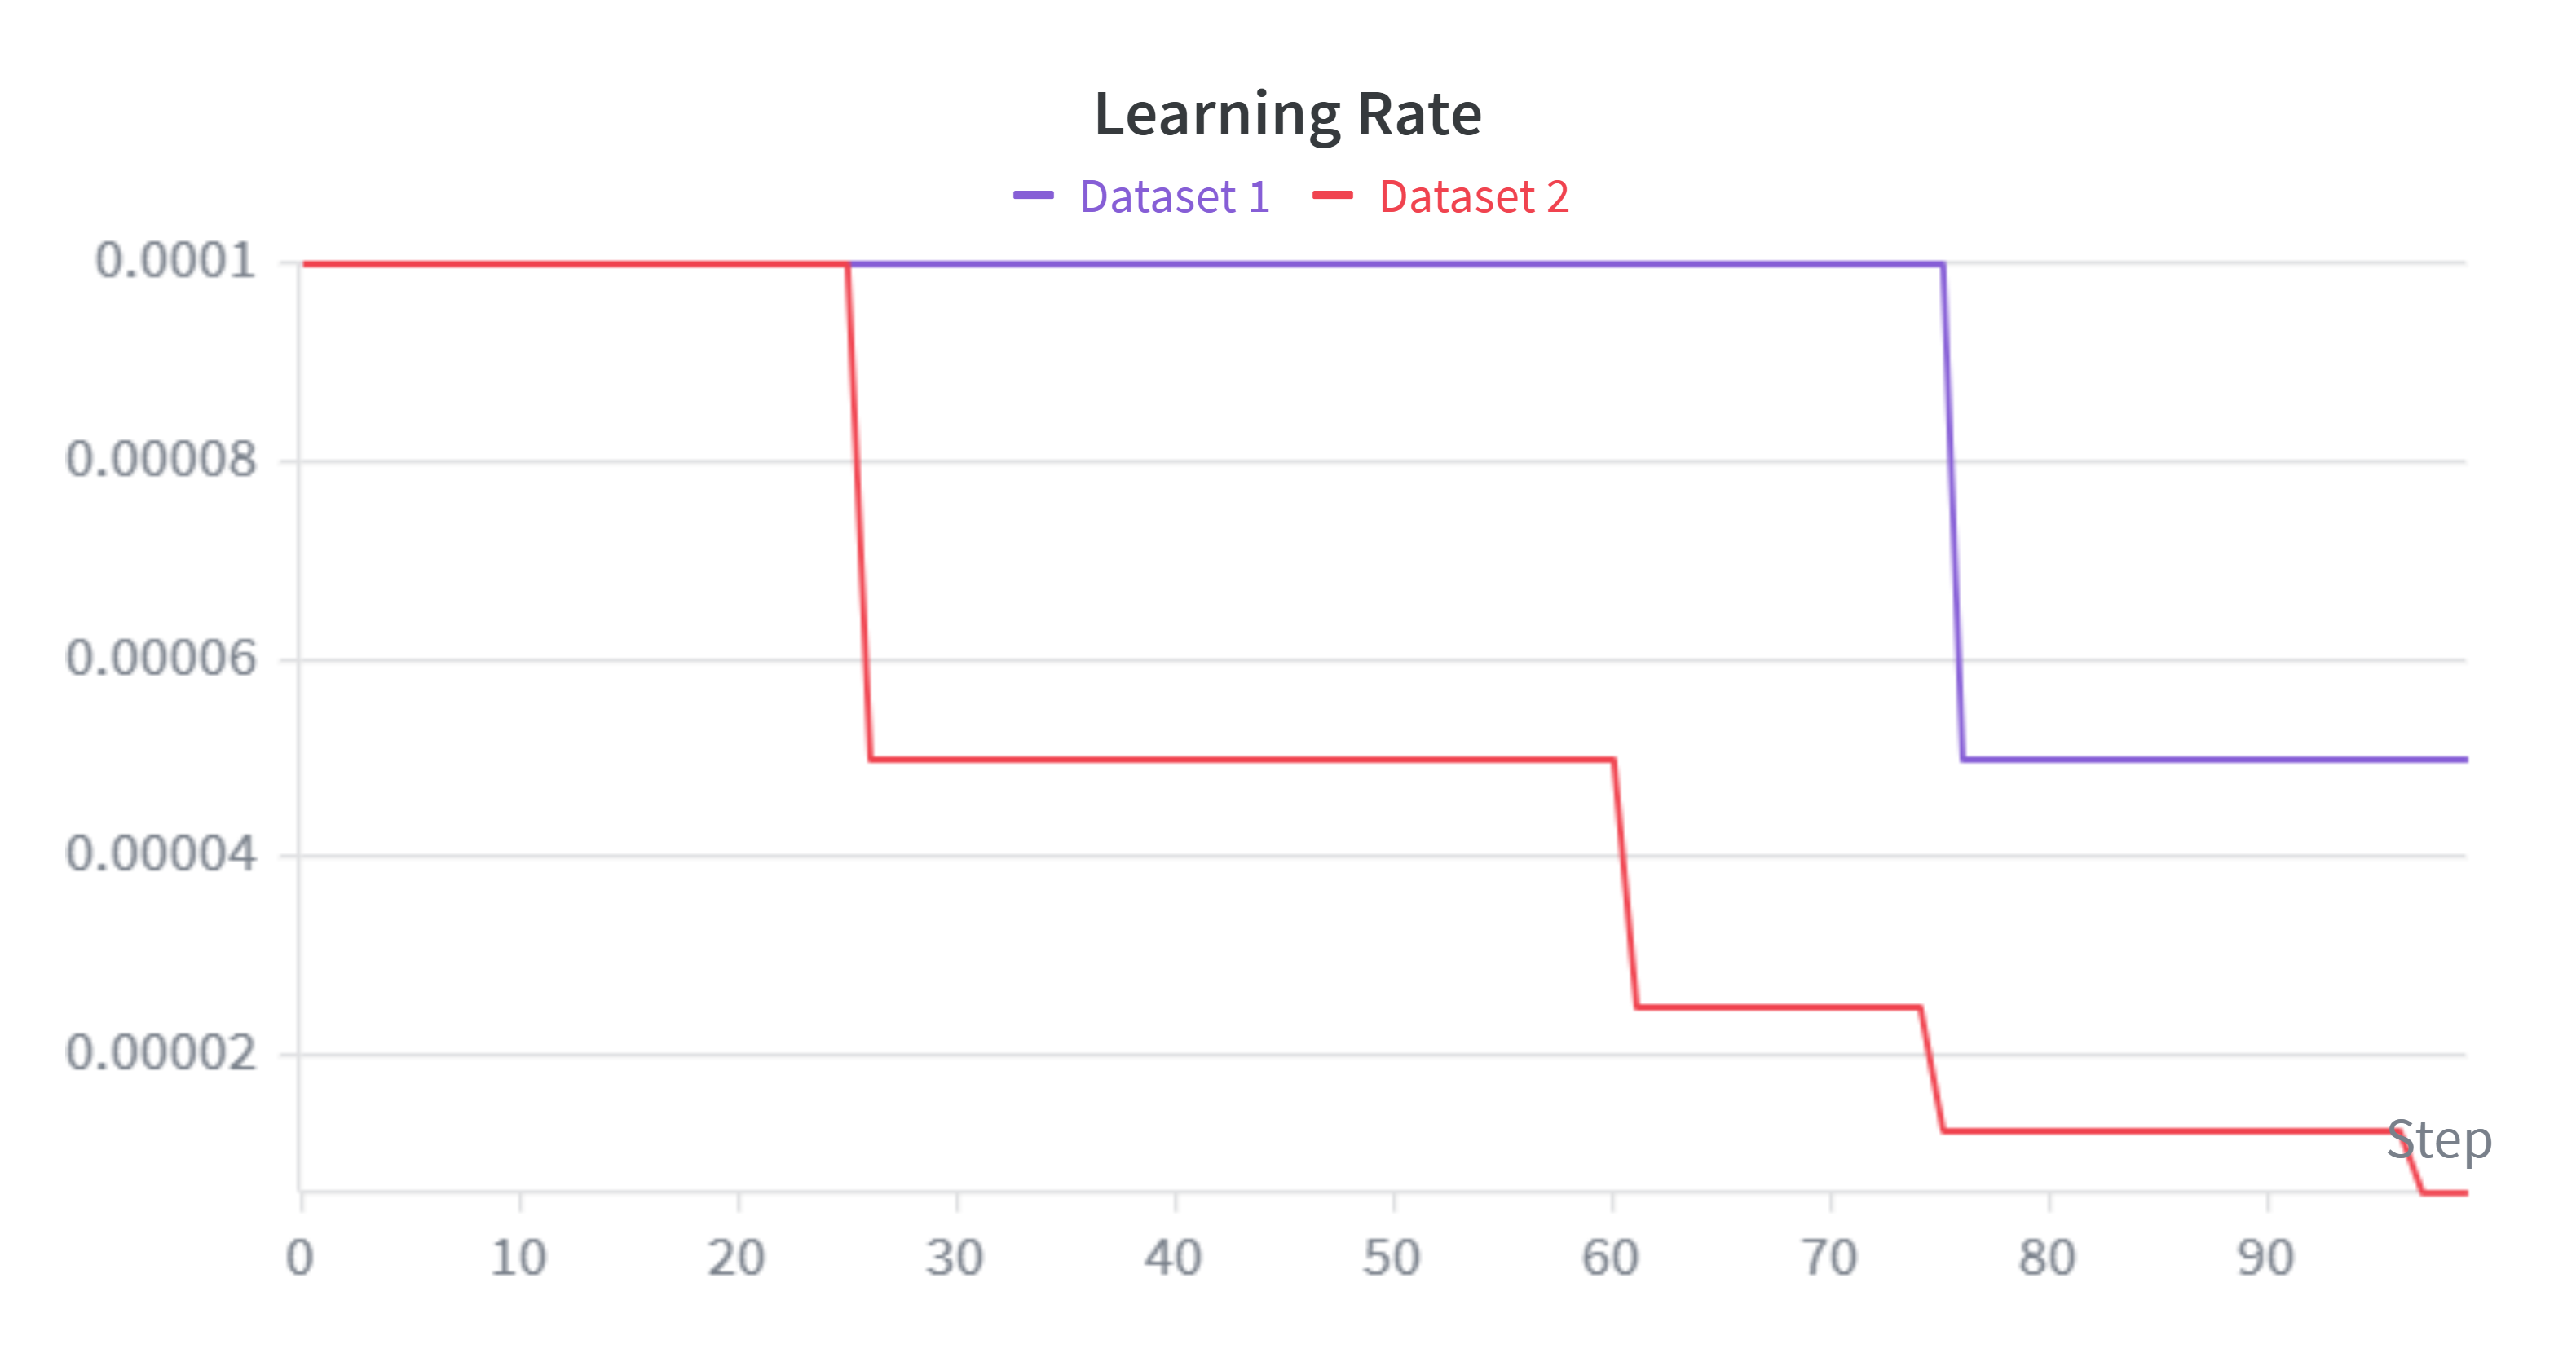
\includegraphics[width=0.95\linewidth]{figures/LearningRate.png}
  \caption{Learning rate schedule}
  \label{fig:lr_compare}
\end{figure}

\subsubsection{Dataset Comparison}
\label{subsubsec:dataset_comparison}
\label{sec:results_comparison}

% Table moved to Conclusion
The single-process model achieves a $4\times$ reduction in MRE ($7.7\times \to 1.91\times$) despite having access to fewer than one-fifth of the distinct process configurations. This confirms that generality goal described in Section~\ref{sec:experiment}, a single model spanning all process nodes, cannot be achieved without sacrificing accuracy: the model's capacity is consumed by inter-process discrimination rather than intra-circuit current prediction. The per-process architecture described in Section~\ref{sec:fw_perprocess} is therefore adopted as the primary path forward.

\section{Conclusion}
\label{sec:conclusion}

\begin{table*}[tp]
\centering
\captionsetup{justification=centering}
\begin{tabular}{|l|c|c|c|}
\hline
\textbf{Training Set} & \textbf{Processes} & \textbf{Final Test L1} & \textbf{Final MRE} \\
\hline
Dataset~2 (multi-process) & 9 & 0.187 & $7.7\times$ \\
Dataset~1 (single process) & 1 & 0.221 & $\mathbf{1.91\times}$ \\
\hline
\end{tabular}
\caption{Head-to-head comparison of multi-process and single-process training.\\MRE is in physical Amperes on the held-out test set.}
\label{tab:comparison}
\end{table*}

The answers to the questions posed in the Experiment section are: Yes and No.

\textit{Yes.} For a single process (Dataset~1), the model achieves a mean relative error (MRE) of $1.91\times$ on the held-out test set, demonstrating that the GATv2 can predict inter-stage current with sufficient accuracy for practical use in design flows.

\textit{No.} The multi-process model (Dataset~2) achieves an MRE of $7.7\times$, which is $4\times$ worse than the single-process model. This indicates that a single model spanning all process nodes cannot achieve the same accuracy as dedicated per-process models. The correct path forward is to train a separate model for each process technology.

This work demonstrates that a GATv2 graph neural network can be trained to predict the inter-stage peak current (I\_target) of a cascaded CMOS inverter chain from transistor dimensions and process parameters alone, without any SPICE simulation at inference time. Two training regimes were evaluated: a multi-process model trained on Dataset~2 (nine process technologies, 112,500 simulations) and a single-process model trained on Dataset~1 (22\,nm HP, 100,000 simulations).

The multi-process model (Dataset 2) converged to a test L1 loss of 0.187 and an I\_target MRE of $7.7\times$ after 100 epochs, with the \texttt{ReduceLROnPlateau} scheduler halving the learning rate four times before stalling. This plateau is evidence of a capacity ceiling: a significant portion of the model's expressiveness is consumed distinguishing nine process-technology clusters rather than learning the intra-circuit current mapping.

Training on Dataset~1 removes the 33 BSIM4 process parameters from the feature vector entirely, reducing node feature dimensionality from $\sim$56 to $\sim$10 and eliminating the inter-process discrimination burden. The single-process model (Dataset 1) achieved a final MRE of $1.91\times$, a $4\times$ improvement over the multi-process model, with the learning rate halved only once across 100 epochs, indicating clean and stable convergence. The comparison in Section~\ref{sec:results_comparison} confirms that the generality goal described in Section~\ref{sec:experiment}, a single model spanning all process nodes, cannot be achieved without a substantial accuracy cost. Accordingly, this work concludes that the correct path forward is one dedicated model per manufacturing process, trained on data generated solely from that process's simulation model.

\subsection{Future Work}
\label{subsec:future_work}

The following future work directions aim to improve the automation, generalizability, and privacy of the current prediction pipeline. Key goals include automating dataset/model generation, integrating feature engineering into data preprocessing, expanding to per-process and multi-design models, and developing privacy-preserving training methods. These steps will enable broader applicability, reproducibility, and secure deployment of the approach in real-world semiconductor design environments.

\subsubsection{Integrated Pipeline}
\label{subsubsec:integrated_pipeline}

Currently, dataset generation (SPICE simulation via SLURM), parsing, and model training are separate manual steps. A single automated flow, triggered by supplying a process model file and a set of design netlists, would run simulations, parse results into the per-process dataset format, and launch training, producing a deployable model checkpoint and an inference endpoint with no manual intervention. This would lower the barrier to adding new process nodes or circuits.

\subsubsection{Integrating Feature Engineering}
\label{subsubsec:feature_label_integration}

Currently, feature engineering (such as categorical encoding and feature standardization) and label normalization (log-scaling and standardization) are performed as part of the model training pipeline. Moving these steps into the dataset generation process would improve reproducibility, simplify the training workflow, and ensure that all downstream users of the dataset apply the same transformations. This approach is common in large-scale machine learning projects, where preprocessing is tightly coupled to dataset versioning.

If feature engineering is performed during dataset generation, the dataset should include both the transformed features and the parameters used for standardization (e.g., means and variances for each feature). This ensures that any future model training or inference can apply the exact same transformations, avoiding data leakage or inconsistencies. Similarly, if label normalization (such as log-scaling and standardization) is moved to dataset generation, the normalization parameters ($\mu$, $\sigma$) must be stored alongside the dataset and used for both training and inverse transformation at evaluation time.

Potential caveats include the need to carefully track and version the preprocessing parameters, especially if the dataset is updated or extended. For maximum flexibility, it may be beneficial to store both raw and processed versions of the data, or to provide scripts that can regenerate the processed dataset from raw simulation outputs using the same transformation logic. Overall, integrating feature engineering and label normalization into dataset generation is a recommended best practice for improving reproducibility and workflow efficiency.

\subsubsection{Per-Process Models}
\label{subsubsec:per_process_models}
\label{sec:fw_perprocess}

This work validated the per-process training approach using the 22\,nm HP process only. The natural next step is to generate datasets for each of the remaining eight process nodes and train a dedicated model for each, following the same pipeline. Comparing the final I\_target MRE across all nine models will confirm whether the accuracy improvement observed for 22\,nm HP generalises across process technologies and will identify any processes that may require additional data or architectural tuning.

\subsubsection{Multi-Design Datasets}
\label{subsubsec:multi_design_datasets}

The current datasets contain only the two-inverter chain (2inv). A more robust evaluation requires simulation data from multiple circuit designs (e.g.\ ring oscillators, NAND/NOR gates, full adder stages). Expanding the dataset to cover several designs and retraining the per-process models will test whether the GATv2 graph representation generalizes across circuit topologies, which is a prerequisite for deployment in a real place-and-route flow.

\subsubsection{Privacy-Preserving Training}
\label{subsubsec:privacy_preserving}

The per-process model architecture maps naturally onto the real-world privacy boundary: a single model trained on data from one foundry's process model encodes only that foundry's IP. In commercial semiconductor design, process model files (\texttt{.pm}) are delivered under strict NDA. Three approaches are under consideration for hardening the training pipeline:

\textbf{Split Encoder Architecture (most practical).}
The foundry trains a small private encoder locally that maps raw BSIM4 parameters to a compact fixed-size embedding (e.g.\ 16 floats). The foundry shares only the embedding vectors alongside simulation I/O pairs. The design house trains the GATv2 layers on \texttt{(W, L, VDD, Temp, Skew, process\_embedding)} $\rightarrow$ I\_target. The encoder weights remain at the foundry; neither the model weights nor the embeddings alone are sufficient to recover the original process parameters.

\textbf{Federated Learning with Differential Privacy.}
The foundry runs simulations locally and shares only gradient updates, never raw data. Calibrated Gaussian noise is added to gradients before transmission (DP-SGD \cite{abadi2016deep}), providing a formal privacy budget $\varepsilon$. The PyTorch Opacus library supports DP-SGD and would integrate directly with the existing training loop.

\textbf{Secure Inference via Trusted Execution.}
Model weights are encrypted at rest and decrypted only inside a Trusted Execution Environment (Intel SGX or AMD SEV) at inference time, protecting both the foundry's process information encoded in the weights and the design house's model IP.

\section*{Acknowledgements}
\label{sec:acknowledgements}

The author would like to thank Alexander La Chapelle and Jonathan Guzman for their contribution to the original version of this paper for our Deep Learning class Oregon State University.  The author would also like to thank Dr. Fuxin Li, the course instruction, for his feedback, which directly led to these improvements.  The original paper can be found here: \url{https://web.engr.oregonstate.edu/~jonesm25/writing/Current%20Prediction%20in%20Analog%20Integrated%20Circuits.pdf}

\bibliographystyle{plainurl}
\bibliography{Bibliography}

% ================= APPENDIX: Python Code =================
\clearpage
\appendix
\onecolumn

\section*{Appendix}
\label{sec:appendix}

All code and netlists used in this work are included below for report completeness. The GitHub repository can be found here: \url{https://github.com/YosemiteSamurai/CurrentPrediction}.

\subsection*{Spice Netlists}
\label{appendix:netlists}

\subsubsection*{2inv.sp}
\label{netlist:2inv}
\verbatiminput{netlists/2inv.sp}

\subsubsection*{template.sp}
\label{netlist:template}
\verbatiminput{netlists/template.sp}

\subsection*{Python Code}
\label{appendix:python}

\subsubsection*{dataset.py}
\label{code:dataset}
\verbatiminput{python/dataset.py}

\subsubsection*{extract\_model\_params.py}
\label{code:extract_model_params}
\verbatiminput{python/extract_model_params.py}

\subsubsection*{gan.py}
\label{code:gan}
\verbatiminput{python/gan.py}

\subsubsection*{graph.py}
\label{code:graph}
\verbatiminput{python/graph.py}

\subsubsection*{models.py}
\label{code:models}
\verbatiminput{python/models.py}

\subsubsection*{parse\_results.py}
\label{code:parse_results}
\verbatiminput{python/parse_results.py}

\subsubsection*{predict.py}
\label{code:predict}
\verbatiminput{python/predict.py}

\subsubsection*{run\_sims.py}
\label{code:run_sims}
\verbatiminput{python/run_sims.py}

\subsubsection*{sweep.py}
\label{code:sweep}
\verbatiminput{python/sweep.py}

\twocolumn
\end{document}
